% Provenance (never printed): see sources/outline_sources.md (Year 3: elastic waves
% recalled from the physics books; rays in a spherical Earth; travel-time tables;
% surface waves and dispersion; normal modes, told; linear inverse problems and
% seismic tomography). Brief: sources/book5/BRIEFS.md, ch. 1. Curves from
% figdata/bachelor-3/ray_tracing.py, love_dispersion.py, tomo_checkerboard.py;
% exercise and problem values in the Book 5 scratch calculator calc/ch01.py.
\chapter{Seismologie en aardbeeldvorming}\label{ch:b3:seismology-imaging}

Op 22 mei 1960, om 19:11 uur wereldtijd, vond de sterkste sinds 1900 geregistreerde
aardbeving plaats en brak de subductiezone voor de kust van zuidelijk Chili, met een magnitude van 9.5.
% ledger: usgs5:chile1960
Haar P-golven bereikten stations aan de andere kant van de planeet ongeveer twintig minuten
later; haar oppervlaktegolven gingen meermaals rond de aardbol; en
dagenlang daarna registreerden de traagste instrumenten de hele Aarde trillend met
perioden van bijna een uur, als een aangeslagen klok. Elk van deze signalen draagt
informatie over de gesteenten die het doorkruiste. Uit de aankomsttijden van miljoenen
van dergelijke golven, afgelezen op duizenden stations, hebben seismologen niet alleen
het gelaagde model van de Aarde dat hieronder wordt opgefrist, maar ook driedimensionale beelden van
de mantel, waarin dalende slabs en opstijgende mantelpluimen verschijnen als gebieden waar
de golven iets sneller of trager dan gemiddeld reizen. Dit hoofdstuk laat zien hoe:
hoe stralen door een bolvormige Aarde reizen, hoe oppervlaktegolven de korst
en mantel via hun dispersie onderzoeken, hoe de vrije trillingen van de hele
planeet worden beschreven, en hoe enkele duizenden looptijden worden omgezet
in een beeld door een lineair \omterm{def:b3:seismology-imaging:inverse}{invers probleem} op te lossen.

\begin{recall}
In een isotroop elastisch vast medium reizen twee soorten lichaamsgolven: P-golven, met de
snelheid $\alpha = \sqrt{(K + \tfrac43\mu)/\rho}$, en S-golven, met de
snelheid $\beta = \sqrt{\mu/\rho}$, waarbij $K$ en $\mu$ de volume- en schuifmoduli zijn
en $\rho$ de dichtheid; S-golven doorkruisen geen vloeistof (natuurkunde, derde
jaar universiteit, in het hoofdstuk over continuümelasticiteit). Een golf waarvan de fasesnelheid
van de frequentie afhangt, is dispersief; haar energie reist met de
groepssnelheid $U = \mathrm d\omega/\mathrm dk$ (natuurkunde, tweede jaar universiteit, over
golven). Een begrensd elastisch lichaam trilt vrij in een discrete reeks
normaalmodi (hetzelfde deel). De epicentrale afstand $\Delta$ van een station is de hoek
in het middelpunt van de Aarde tussen het epicentrum en het station; de
looptijdkromme geeft de tijd van de eerste aankomst als functie van $\Delta$, en de kern werpt een
schaduwzone voor directe P-golven (Boek~2, leerjaar~11). Het referentiemodel van de aarde,
de seismische discontinuïteiten en de kopgolf kwamen aan bod in Boek~3,
in het hoofdstuk over de gelaagde Aarde. Kleinste kwadraten en de gaussische
foutenwet komen uit de wiskundeboeken.
\end{recall}

\section{Stralen in een bolvormige Aarde}

Een seismisch golffront, ver van zijn bron en in een medium waarvan de eigenschappen
over een golflengte langzaam veranderen, kan worden gevolgd via zijn stralen: de krommen
die overal loodrecht op het golffront staan en waarlangs de energie reist. In een
medium met uniforme snelheid zijn de stralen recht; waar de snelheid verandert,
buigen ze af volgens de wet van Snell voor breking. In de Aarde hangen de snelheden
vooral af van de diepte, zodat een eerste model bolsymmetrisch is: de snelheid $v(r)$ van de
beschouwde golf (P of S) is een functie van de straal $r$ alleen.

\begin{theorem}[De wet van Snell in een bolvormige Aarde]\label{thm:b3:seismology-imaging:snell}
In een bolsymmetrische Aarde met golfsnelheid $v(r)$ zij $i$ de hoek
tussen een straal en de radiale richting in het punt op afstand $r$ van het middelpunt. Langs de gehele straal,
\[
  \frac{r\sin i}{v(r)} = p
\]
is constant.
\end{theorem}

\begin{proof}
Vervang de Aarde door dunne concentrische schillen, elk met een uniforme snelheid. Binnen een
schil is de straal een rechte lijn; een rechte lijn op afstand $d$ van het
middelpunt snijdt de bol met straal $r$ onder een hoek $i$ met
$r\sin i = d$ (de rechthoekige driehoek gevormd door het middelpunt, het voetpunt van de
loodlijn en het punt), zodat $r\sin i$ aan de bovenkant en aan de
onderkant van de schil gelijk is. Op de grens van straal $r$ tussen twee schillen met
snelheden $v_1$ en $v_2$ geeft de wet van Snell $\sin i_1/v_1 = \sin i_2/v_2$, dus
$r\sin i/v$ is over de grens continu. Binnen een schil is $v$ constant en
$r\sin i$ is constant, dus is ook $r\sin i/v$ daar eveneens constant. Het is dus
langs de gehele straal constant; laat men de dikte van de schillen naar nul gaan
dan volgt het resultaat voor een continue $v(r)$.
\end{proof}

\begin{definition}[Straalparameter, keerpunt]\label{def:b3:seismology-imaging:ray-parameter}
De constante $p = r\sin i/v(r)$ van een straal in een bolsymmetrische Aarde heet
haar \emph{straalparameter}\index{straalparameter}, in seconden per radiaal. Aan het
oppervlak is $p = R\sin i_0/v_0$, waarbij $i_0$ de vertrekhoek is en $v_0$
de snelheid aan het oppervlak. Het punt waar de straal horizontaal loopt ($i = \ang{90}$)
is het \emph{keerpunt (van een seismische straal)}\index{keerpunt (van een seismische straal)},
op de straal $r_t$ waar
\[
  \frac{r_t}{v(r_t)} = p .
\]
Daaronder stijgt de straal weer op, symmetrisch ten opzichte van de straal door het
keerpunt.
\end{definition}

Schrijf $\eta(r) = r/v(r)$. Een straal met parameter $p$ kan alleen bestaan waar
$\eta \ge p$, want $\sin i = p/\eta \le 1$. Als $\eta$ met de diepte afneemt, zoals
dat doet in het grootste deel van de mantel, keert elke straal om op de diepte waar $\eta$
is gedaald tot $p$, en stralen die steiler vertrekken (kleinere $p$) keren dieper om.
Waar $\eta$ met de diepte \emph{toeneemt}, doordat de snelheid sterk daalt met
de diepte (dat gebeurt op de kern-mantelgrens, waar de P-snelheid daalt van
13.7 naar \qty{8.0}{km.s^{-1}}), % ledger: ak135:cmb
geen enkele straal kan omkeren: de stralen worden naar beneden gebogen, doorkruisen de laag en komen ver weg weer omhoog.
Zo'n sprong werpt een schaduw aan het oppervlak.

\begin{omfigure}
\begin{tikzpicture}[font=\small, x=1.6cm, y=1.6cm]
% concentric shells, centre O at (0,-9) (outside the picture); ray computed by
% Snell's law for v = 1, 1.35, 1.68 and a take-off angle of 30 deg
% (scratch calc/shells_fig.py)
\coordinate (O) at (0,-9);
\fill[blue!6] ($(O)+(62:9)$) arc (62:118:9) -- ($(O)+(118:8.4)$) arc (118:62:8.4) -- cycle;
\fill[blue!12] ($(O)+(62:8.4)$) arc (62:118:8.4) -- ($(O)+(118:7.8)$) arc (118:62:7.8) -- cycle;
\fill[blue!18] ($(O)+(62:7.8)$) arc (62:118:7.8) -- ($(O)+(118:7.0)$) arc (118:62:7.0) -- cycle;
\draw[thick] ($(O)+(62:9)$) arc (62:118:9);
\foreach \r in {8.4, 7.8} {\draw[gray] ($(O)+(62:\r)$) arc (62:118:\r);}
\draw[gray, densely dashed] ($(O)+(62:7.0)$) arc (62:118:7.0);
\node[anchor=east] at ($(O)+(118.3:9)$) {$R$};
\node[anchor=east, gray!60!black] at ($(O)+(118.3:8.4)$) {$r_1$};
\node[anchor=east, gray!60!black] at ($(O)+(118.3:7.8)$) {$r_2$};
\node[blue!60!black] at ($(O)+(64:8.7)$) {$v_0$};
\node[blue!60!black] at ($(O)+(64:8.1)$) {$v_1$};
\node[blue!60!black] at ($(O)+(64:7.4)$) {$v_2$};
\coordinate (A) at (-3.295,-0.625);
\coordinate (B) at (-2.746,-1.062);
\coordinate (C) at (-1.920,-1.440);
\coordinate (T) at (0,-1.440);
\coordinate (C') at (1.920,-1.440);
\coordinate (B') at (2.746,-1.062);
\coordinate (A') at (3.295,-0.625);
% radii at the source and at the first boundary, towards the centre
\draw[densely dashed] ($(A)!-0.04!(O)$) -- ($(A)!0.12!(O)$);
\draw[densely dashed] ($(B)!-0.04!(O)$) -- ($(B)!0.11!(O)$);
\draw[densely dashed] (T) -- (0,-2.15);
\draw[very thick, red!70!black] (A) -- (B) -- (C) -- (T) -- (C') -- (B') -- (A');
\pic[draw, angle radius=0.75cm, pic text={$i_0$}, angle eccentricity=1.4] {angle = O--A--B};
\pic[draw, angle radius=0.65cm, pic text={$i_1$}, angle eccentricity=1.45] {angle = O--B--C};
\fill (A) circle (2pt) node[above left=1pt] {bron};
\fill (A') circle (2pt) node[above right=1pt] {station};
\fill[red!70!black] (T) circle (1.6pt);
\node[anchor=north west, red!70!black] at (0.05,-1.47) {keerpunt, $r_t/v_2 = p$};
\node[anchor=north, font=\scriptsize] at (0,-2.15) {naar het middelpunt $O$};
\end{tikzpicture}

\par\smallskip{\small Een straal in een bolvormige aarde, opgedeeld in schillen met uniforme
snelheid (schematisch, niet op schaal). In elke schil is de straal recht; bij elke
grens breekt hij volgens de wet van Snellius, weg van de straal wanneer de snelheid
naar beneden toeneemt. De grootheid $r\sin i/v$ behoudt langs de straal dezelfde
waarde $p$; de straal is horizontaal in zijn keerpunt, waar $r/v = p$, en stijgt
daarna symmetrisch weer op.}
\label{fig:b3:seismology-imaging:shells}
\end{omfigure}

De \omterm{def:b3:seismology-imaging:ray-parameter}{straalparameter} is niet alleen een constante van de straal: ze kan worden afgelezen
van de looptijdkromme.

\begin{theorem}[Helling van de looptijdkromme]\label{thm:b3:seismology-imaging:benndorf}
Zij $T(\Delta)$ de looptijd van een straal van een bronpunt aan het oppervlak naar een
station aan het oppervlak op de epicentrale afstand $\Delta$ (in radialen). Dan geldt
\[
  \frac{\mathrm dT}{\mathrm d\Delta} = p ,
\]
de \omterm{def:b3:seismology-imaging:ray-parameter}{straalparameter} van de straal die bij $\Delta$ aankomt.
\end{theorem}

\begin{proof}
Beschouw twee naburige stralen vanuit dezelfde bron, die aan het oppervlak aankomen
bij $\Delta$ en $\Delta + \mathrm d\Delta$, beide onder de invalshoek $i_0$ ten opzichte
van de straal naar het middelpunt. Het golffront door het eerste punt staat loodrecht
op de stralen; de tweede straal moet na het kruisen van dat golffront nog de zijde
afleggen van een kleine rechthoekige driehoek waarvan de schuine zijde de boog
$R\,\mathrm d\Delta$ langs het oppervlak is en waarvan de hoek tegenover die zijde
$i_0$ is: een lengte $R\,\mathrm d\Delta\,\sin i_0$, met de snelheid $v_0$. Dus
$\mathrm dT = R\sin i_0\,\mathrm d\Delta/v_0 = p\,\mathrm d\Delta$.
\end{proof}

De stelling is de bolvormige vorm van het verband $\mathrm dT/\mathrm dx = 1/c$
tussen de helling van een looptijdkromme en de schijnbare snelheid $c$ langs het
oppervlak. De twee functies $T(p)$ en $\Delta(p)$ kunnen worden geschreven als integralen
over het snelheidsprofiel.

\begin{proposition}[Looptijd en afstand als integralen]\label{prop:b3:seismology-imaging:integrals}
Met $\eta = r/v(r)$, dat met de diepte afneemt, bereikt de straal met parameter $p$ die
keert bij $r_t$
\[
  \Delta(p) = 2\int_{r_t}^{R}\frac{p\,\mathrm dr}{r\sqrt{\eta^2 - p^2}},
  \qquad
  T(p) = 2\int_{r_t}^{R}\frac{\eta^2\,\mathrm dr}{r\sqrt{\eta^2 - p^2}},
\]
en de intercepttijd $\tau(p) = T - p\Delta$ is
$\tau(p) = 2\int_{r_t}^{R}\sqrt{\eta^2 - p^2}\,\mathrm dr/r$.
\end{proposition}

\begin{proof}
Langs een element van de straal met lengte $\mathrm ds$ verandert de straal met
$\mathrm dr = \cos i\,\mathrm ds$ en de hoek in het middelpunt met
$\mathrm d\Delta = \sin i\,\mathrm ds/r$, dus $\mathrm d\Delta = \tan i\,\mathrm dr/r$.
Met $\sin i = p/\eta$ geldt $\tan i = p/\sqrt{\eta^2 - p^2}$, wat de eerste integraal
geeft voor de dalende helft; de stijgende helft is hetzelfde. De tijd is
$\mathrm dT = \mathrm ds/v = \mathrm dr/(v\cos i)$, en $1/v = \eta/r$,
$1/\cos i = \eta/\sqrt{\eta^2 - p^2}$. Ten slotte heeft $T - p\Delta$ als integrand
$(\eta^2 - p^2)/(r\sqrt{\eta^2 - p^2})$.
\end{proof}

Deze integralen zijn de manier waarop een \omterm{def:b3:seismology-imaging:tables}{looptijdtabel} uit een model wordt berekend. Het
raytracingscript van dit hoofdstuk doet dezelfde som over schillen van 2~km van het
referentiemodel PREM, % ledger: data:prem
en controleert het op twee manieren: in een bol met uniforme snelheid, waar de stralen
koorden zijn en $T = 2R\sin(\Delta/2)/v$ exact geldt (oefening 5), en tegen
\cref{thm:b3:seismology-imaging:benndorf}, die het niet gebruikt.

\begin{omfigure}
\begin{tikzpicture}
\begin{axis}[axis equal image, hide axis, width=0.66\linewidth,
  xmin=-1500, xmax=6700, ymin=-6700, ymax=6700, clip=false]
\addplot[draw=none, fill=gray!8, domain=0:360, samples=181] ({6371*cos(x)},{6371*sin(x)});
\addplot[black, thick, domain=0:360, samples=181] ({6371*cos(x)},{6371*sin(x)});
\addplot[orange!70!black, fill=orange!12, domain=0:360, samples=181] ({3480*cos(x)},{3480*sin(x)});
\addplot[orange!80!black, fill=orange!35, domain=0:360, samples=121] ({1221.5*cos(x)},{1221.5*sin(x)});
\addplot[blue!70!black, unbounded coords=jump] table[x=x, y=y] {figdata/out/bachelor-3-ray_tracing-rays-mantle.dat};
\addplot[red!70!black, unbounded coords=jump] table[x=x, y=y] {figdata/out/bachelor-3-ray_tracing-rays-core.dat};
% shadow zone for direct P, from 98.5 deg to the caustic B at 143.8 deg
\addplot[gray!60!black, line width=3pt, opacity=0.5, domain=98.5:143.8, samples=40]
  ({6371*sin(x)},{6371*cos(x)});
\fill (axis cs:0,6371) circle (2.2pt);
\node[anchor=south] at (axis cs:0,6371) {\small bron};
\node[anchor=west, font=\small] at (axis cs:{6371*sin(120)+150},{6371*cos(120)}) {schaduwzone};
\node[anchor=west, font=\scriptsize] at (axis cs:{6371*sin(98.5)+120},{6371*cos(98.5)}) {\ang{98.5}};
\node[anchor=west, font=\scriptsize] at (axis cs:{6371*sin(143.8)+120},{6371*cos(143.8)}) {\ang{143.8}};
\node[font=\scriptsize, orange!50!black] at (axis cs:-1450,1650) {buitenkern};
\draw[orange!50!black, thin] (axis cs:-700,-500) -- (axis cs:-2500,-4300) node[anchor=north, font=\scriptsize] {binnenkern};
\node[font=\scriptsize] at (axis cs:-3300,4200) {mantel};
\end{axis}
\end{tikzpicture}

\par\smallskip{\small P-stralen vanuit een bronpunt aan het oppervlak door het referentiemodel
PREM, getraceerd door schillen van 2~km, voor uittreedhoeken van \ang{2} tot \ang{34}
ten opzichte van de verticaal. Blauw: stralen die in de mantel keren; die bereiken hooguit
\ang{98.5}; ze buigen omhoog omdat de snelheid met de diepte toeneemt, en de knikken
nabij de bovenkant markeren de discontinuïteiten van het model, bij 220, 400 en
\qty{670}{km}.
Rood: stralen die de kern binnengaan, scherp naar beneden gebogen bij de kern-mantelgrens,
waar de snelheid daalt; de stralen die in de buitenkern keren, bereiken het oppervlak
weer pas bij \ang{143.8}. Daartussen ligt de schaduwzone van directe P (grijze
boog), die alleen wordt bereikt door zwakke golven die door de binnenkern gaan of daar
worden weerkaatst.}
\label{fig:b3:seismology-imaging:rays}
\end{omfigure}

De figuur hierboven laat zien wat de stellingen voorspellen. De steilste mantelstraal die
de kern net raakt, bereikt \ang{98.5} in PREM; de volgende straal, een fractie van een
graad steiler, gaat de kern in, wordt naar het middelpunt toe gebroken en komt aan de
andere kant tevoorschijn, voorbij \ang{140}. Door de tijd tegen de afstand uit te zetten
voor elke straal ontstaan de looptijdkrommen hieronder.

De berekende P-looptijden door PREM zijn \qty{273.5}{s} bij \ang{20},
\qty{369.6}{s} bij \ang{30}, \qty{607.2}{s} bij \ang{60} en \qty{779.7}{s} bij
\ang{90}: dertien minuten om een kwart van de aardbol te doorkruisen.
% figdata: bachelor-3-ray_tracing-values (PREM, ledger data:prem)
Werkelijke aankomsten wijken van zo'n kromme hooguit enkele seconden af, en die paar
seconden zijn de gegevens van de tomografie (\cref{sec:b3:seismology-imaging:tomography}).

\begin{definition}[Looptijdtabel]\label{def:b3:seismology-imaging:tables}
Een \emph{looptijdtabel}\index{looptijdtabel} geeft, voor elke seismische
fase (P, S, PKP, PcP, \dots) en elke brondiepte de looptijd als functie van
de epicentrale afstand, berekend uit een sferisch symmetrisch
referentiemodel waarvan de snelheden zelf zijn aangepast aan de tijden van een
grote reeks goed gelokaliseerde aardbevingen. De verschillen met een waargenomen
aankomst vormen het uitgangspunt van aardbevingslokalisatie en van tomografie.
\end{definition}

De tabellen die nu in gebruik zijn, worden berekend uit referentiemodellen die daarvoor
zijn opgebouwd. In het model \texttt{ak135} heeft de korst bijvoorbeeld twee lagen,
met P- en S-snelheden van 5.80 en \qty{3.46}{km.s^{-1}} boven \qty{20}{km} en
6.50 en \qty{3.85}{km.s^{-1}} tot aan de Moho op \qty{35}{km}, waar de
mantel begint met 8.04 en \qty{4.48}{km.s^{-1}}; de kern-mantelgrens ligt
op \qty{2891.5}{km} en de binnenkerngrens op \qty{5153.5}{km}.
% ledger: ak135:discontinuities, ak135:crust
De auteurs omschrijven de bovenmantel zelf als een kunstmatige constructie, ontworpen
om de tijden tot \ang{30} te passen: een gemiddelde, niet de opbouw onder
één bepaalde plek.

\begin{omfigure}
\begin{tikzpicture}
\begin{axis}[omrecord, width=0.84\linewidth, height=0.46\linewidth,
  xmin=0, xmax=180, ymin=0, ymax=27, xtick={0,20,...,180},
  xlabel={epicentrale afstand $\Delta$ (\unit{\degree})},
  ylabel={looptijd (\unit{min})},
  legend style={at={(0.98,0.04)}, anchor=south east, font=\scriptsize}, legend cell align=left]
\addplot[blue!70!black, thick] table[x=delta, y=t] {figdata/out/bachelor-3-ray_tracing-tt-P.dat};
\addlegendentry{P (keerpunt in de mantel)}
\addplot[red!70!black, thick] table[x=delta, y=t] {figdata/out/bachelor-3-ray_tracing-tt-PKP.dat};
\addlegendentry{PKP (buitenkern)}
\addplot[orange!80!black, thick, densely dashed] table[x=delta, y=t] {figdata/out/bachelor-3-ray_tracing-tt-PKIKP.dat};
\addlegendentry{PKIKP (binnenkern)}
\addplot[green!45!black, thick] table[x=delta, y=t] {figdata/out/bachelor-3-ray_tracing-tt-S.dat};
\addlegendentry{S (keerpunt in de mantel)}
\draw[gray, densely dotted] (axis cs:98.5,0) -- (axis cs:98.5,27);
\draw[gray, densely dotted] (axis cs:143.8,0) -- (axis cs:143.8,27);
\node[font=\scriptsize, anchor=north] at (axis cs:121,26.5) {P-schaduw};
\node[font=\scriptsize, anchor=west] at (axis cs:144,16.8) {kaustiek B};
\end{axis}
\end{tikzpicture}

\par\smallskip{\small Looptijden van P, S en de kernfasen vanuit een bron aan het oppervlak,
bron, berekend met PREM door de integralen van
\cref{prop:b3:seismology-imaging:integrals} over schillen van 2 km op te tellen. De P-kromme
eindigt bij \ang{98.5}; haar helling, de \omterm{def:b3:seismology-imaging:ray-parameter}{straalparameter}, neemt af met de afstand. Onder
\ang{40} heeft zij meerdere, elkaar overlappende takken (triplicaties): stralen die keren
in de zwakke gradiënt tussen de Moho en \qty{220}{km} reizen ver, tot ongeveer
\ang{39}, voordat de stralen die aan de discontinuïteiten van het model worden teruggekaatst, op
220, 400 en \qty{670}{km}, het overnemen; de eerste aankomst is altijd de laagste tak.
De PKP-kromme vouwt terug bij de kaustiek B, bij \ang{143.8}, en haar
korte tak bevat ook de stralen die aan de binnenkerngrens worden teruggekaatst.
De S-kromme (stralen die keren in de mantel; de S-golven die van de kern weerkaatst
worden weggelaten) eindigt nabij \ang{102}: S kruist de vloeibare buitenkern niet.}
\label{fig:b3:seismology-imaging:tt}
\end{omfigure}

\begin{proposition}[Herglotz--Wiechert-inversie]\label{prop:b3:seismology-imaging:herglotz}
Veronderstel dat $\eta = r/v(r)$ over de bemonsterde stralen strikt met de diepte afneemt
en de looptijdkromme $T(\Delta)$ bekend is, zodat $p(\Delta) =
\mathrm dT/\mathrm d\Delta$ bekend is. Dan heeft de straal met parameter $p_1$, die
het oppervlak bereikt bij $\Delta_1$, haar keerpunt op de straal
\[
  r_1 = R\,\exp\!\left(-\frac1\pi\int_0^{\Delta_1}
  \operatorname{arccosh}\frac{p(\Delta)}{p_1}\,\mathrm d\Delta\right),
\]
waarbij de snelheid $v(r_1) = r_1/p_1$ is. De \emph{Herglotz--Wiechert
inversie}\index{Herglotz--Wiechert-inversie} herleidt $v(r)$ zo,
punt voor punt, uit de looptijdkromme.
\end{proposition}
\admitted

De formule volgt uit de integraal van $\Delta(p)$ in
\cref{prop:b3:seismology-imaging:integrals}, een Abelse integraalvergelijking
voor de onbekende $r(\eta)$; de inversie ervan wordt hier aangenomen.
Oefening 12 toetst haar op de uniforme bol. Twee voorwaarden beperken haar. Zij vereist
dat $\eta$ met de diepte afneemt: een laag met lage snelheid maakt een gat in de
looptijdkromme, en de inversie kan niet in de laag kijken. En zij vereist
de hele kromme, inclusief de latere takken van elke triplicatie, die
moeilijk te kiezen zijn op een seismogram. Deze beperkingen zijn de reden dat de referentiemodellen nu
worden opgebouwd met voorwaartse modellering en kleinste kwadraten (\cref{sec:b3:seismology-imaging:inverse}).

\section{Oppervlaktegolven}

Een vrij oppervlak vangt golven op. Nabij het oppervlak van een halfruimte kunnen P- en S-bewegingen
in het verticale vlak van voortplanting samenvoegen tot een golf die langs
het oppervlak loopt en met de diepte afneemt; en waar een langzame laag op sneller gesteente ligt,
worden horizontale schuifgolven in de laag gevangen door totale reflectie.

\begin{definition}[Rayleighgolf, Lovegolf]\label{def:b3:seismology-imaging:surface-waves}
Een \emph{Rayleighgolf}\index{Rayleighgolf} is een oppervlaktegolf waarvan de deeltjesbeweging
ligt in het verticale vlak dat de voortplantingsrichting bevat:
P- en verticaal gepolariseerde S-bewegingen, gekoppeld door het vrije oppervlak, met een
elliptische deeltjesbeweging, retrograde aan het oppervlak van een uniforme halfruimte,
waarvan de amplitude met de diepte afneemt over ongeveer één golflengte. Een \emph{Love
golf}\index{Lovegolf} is een oppervlaktegolf waarvan de deeltjesbeweging horizontaal is
en loodrecht staat op de voortplantingsrichting: horizontaal gepolariseerde S-golven die
gevangen zijn in lagen die langzamer zijn dan het gesteente eronder.
\end{definition}

Op een uniforme halfruimte met $\lambda = \mu$ (een Poisson-vaste stof) reist de
\omterm{def:b3:seismology-imaging:surface-waves}{Rayleighgolf} met $0.9194\,\beta$ en disperseert zij niet (oefening 6). Een \omterm{def:b3:seismology-imaging:surface-waves}{Lovegolf}
kan op een uniforme halfruimte helemaal niet bestaan: zij heeft de gelaagdheid nodig, en haar
snelheid ligt tussen de S-snelheden van de laag en van het gesteente eronder.

\begin{omfigure}
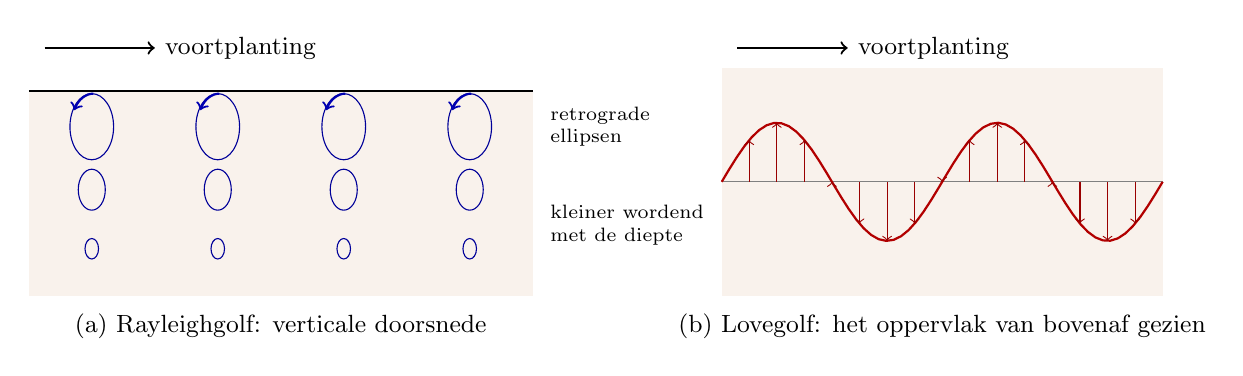
\begin{tikzpicture}[font=\small, x=1cm, y=1cm]
% Rayleigh: vertical section
\fill[brown!10] (0,0) rectangle (6.4,-2.6);
\draw[thick] (0,0) -- (6.4,0);
\draw[->, thick] (0.2,0.55) -- (1.6,0.55) node[right] {voortplanting};
\foreach \x/\s in {0.8/1, 2.4/-1, 4.0/1, 5.6/-1} {
  \foreach \z/\a in {-0.45/0.42, -1.25/0.26, -2.0/0.13} {
    \draw[blue!60!black] (\x,\z) ellipse ({0.66*\a} and {\a});
  }
}
\foreach \x in {0.8, 2.4, 4.0, 5.6} {
  \draw[->, blue!70!black, thick] (\x+0.02,-0.03) arc (90:150:{0.28} and {0.42});
}
\node[anchor=north] at (3.2,-2.7) {(a) Rayleighgolf: verticale doorsnede};
\node[anchor=west, font=\scriptsize, align=left] at (6.5,-0.45) {retrograde\\ellipsen};
\node[anchor=west, font=\scriptsize, align=left] at (6.5,-1.7) {kleiner wordend\\met de diepte};
% Love: plan view of the surface
\begin{scope}[xshift=8.8cm]
\fill[brown!10] (0,0.3) rectangle (5.6,-2.6);
\draw[->, thick] (0.2,0.55) -- (1.6,0.55) node[right] {voortplanting};
\draw[gray, thin] (0,-1.15) -- (5.6,-1.15);
\draw[red!70!black, thick, domain=0:5.6, samples=60] plot (\x,{-1.15+0.75*sin(\x*360/2.8)});
\foreach \x in {0.35,0.7,...,5.3} {
  \pgfmathsetmacro{\d}{0.75*sin(\x*360/2.8)}
  \draw[->, red!60!black] (\x,-1.15) -- (\x,{-1.15+\d});
}
\node[anchor=north] at (2.8,-2.7) {(b) Lovegolf: het oppervlak van bovenaf gezien};
\end{scope}
\end{tikzpicture}

\par\smallskip{\small Deeltjesbewegingen van de twee oppervlaktegolven (schematisch).
(a) Een \omterm{def:b3:seismology-imaging:surface-waves}{Rayleighgolf} beweegt de grond in het verticale vlak van de voortplanting,
langs ellipsen die aan de bovenkant, nabij het oppervlak, naar achteren draaien (retrograd) en
met de diepte kleiner worden. (b) Een \omterm{def:b3:seismology-imaging:surface-waves}{Lovegolf} beweegt de grond horizontaal, dwars op de
voortplantingsrichting: de pijlen tonen de verplaatsing op één moment
langs een lijn van het oppervlak.}
\label{fig:b3:seismology-imaging:particle-motion}
\end{omfigure}

\begin{theorem}[Dispersie van Lovegolven in een laag op een halfruimte]\label{thm:b3:seismology-imaging:love}
Een laag met dikte $H$, afschuifmodulus $\mu_1$ en S-snelheid $\beta_1$ ligt op een
halfruimte met afschuifmodulus $\mu_2$ en S-snelheid $\beta_2 > \beta_1$. Een \omterm{def:b3:seismology-imaging:surface-waves}{Lovegolf}
met hoekfrequentie $\omega$ en golfgetal $k$ plant zich voort met de
fasesnelheid $c = \omega/k$, $\beta_1 < c < \beta_2$, dan en slechts dan als
\[
  \tan\!\left(kH q_1\right) = \frac{\mu_2 q_2}{\mu_1 q_1},
  \qquad q_1 = \sqrt{\frac{c^2}{\beta_1^2} - 1},\quad
  q_2 = \sqrt{1 - \frac{c^2}{\beta_2^2}} .
\]
De fundamentele modus is de wortel met $0 < kHq_1 < \pi/2$; de boventonen hebben
$kHq_1$ in $(n\pi, n\pi + \pi/2)$.
\end{theorem}

\begin{proof}
Neem $x$ langs de voortplanting, $y$ horizontaal dwars daarop en $z$ naar beneden vanaf
het vrije oppervlak, en zoek een verplaatsing
$u_y = f(z)\,e^{i(kx - \omega t)}$, de andere componenten nul. Elke laag
voldoet aan de golfvergelijking $\partial^2 u_y/\partial t^2 = \beta^2\nabla^2 u_y$, dus
$f'' = -k^2\left(c^2/\beta^2 - 1\right) f$. In de laag geldt $c > \beta_1$, en
$f = A\cos(kq_1z) + B\sin(kq_1z)$. In de halfruimte geldt $c < \beta_2$, en de
oplossing die op diepte begrensd blijft is $f = C\,e^{-kq_2(z - H)}$.
De afschuifspanning op een horizontaal vlak is $\mu\,\partial u_y/\partial z$.
Aan het vrije oppervlak verdwijnt zij: $f'(0) = 0$, dus $B = 0$. Bij $z = H$ zijn de
verplaatsing en de spanning continu:
\[
  A\cos(kq_1H) = C, \qquad -\mu_1 A\,kq_1\sin(kq_1H) = -\mu_2\,kq_2\,C .
\]
Deling van de tweede vergelijking door de eerste levert het resultaat. Omdat het
rechterlid positief is, ligt $kHq_1$ in een kwartperiode waarin de
tangens positief is; het kleinste zo'n interval geeft de fundamentele modus.
\end{proof}

Voor een gegeven periode wordt de vergelijking voor $c$ opgelost met bisectie; de
groepssnelheid volgt uit $U = \mathrm d\omega/\mathrm dk$. Bij korte perioden
($kH$ groot) ligt de wortel dicht bij $c = \beta_1$: de golf leeft in de laag. Bij
lange perioden ($kH \to 0$) moet $kHq_1 \to 0$ gaan, met ook het rechterlid
klein, wat $c \to \beta_2$ afdwingt: de golf reikt diep in de
halfruimte en reist met diens snelheid. Tussen de twee stijgt de fasesnelheid
gestaag met de periode.

\begin{definition}[Dispersie van oppervlaktegolven]\label{def:b3:seismology-imaging:dispersion}
\emph{Dispersie van oppervlaktegolven}\index{dispersie van oppervlaktegolven} is de afhankelijkheid
van de fase- en groepssnelheden van een Rayleigh- of \omterm{def:b3:seismology-imaging:surface-waves}{Lovegolf} van haar periode. In
een gelaagde aarde ontstaat zij doordat een golf met een langere periode dieper reikt
(voor de fundamentele modus ongeveer een derde van een golflengte) en sneller
gesteente middelt; de dispersiekrommen $c(T)$ en $U(T)$, gemeten tussen een aardbeving
en een station, of tussen twee stations, worden geïnverteerd naar de S-snelheid als
functie van de diepte.
\end{definition}

\begin{omfigure}
\begin{tikzpicture}
\begin{axis}[omrecord, xmode=log, width=0.82\linewidth, height=0.5\linewidth,
  xmin=3, xmax=150, ymin=3.3, ymax=4.6, log basis x=10,
  xtick={3,5,10,20,50,100,150}, xticklabels={3,5,10,20,50,100,150},
  xlabel={periode $T$ (\unit{s})}, ylabel={snelheid (\unit{km.s^{-1}})},
  legend style={at={(0.03,0.62)}, anchor=west}, legend cell align=left]
\addplot[blue!70!black, thick] table[x=period, y=c] {figdata/out/bachelor-3-love_dispersion-curve.dat};
\addlegendentry{fasesnelheid $c$}
\addplot[red!70!black, thick] table[x=period, y=U] {figdata/out/bachelor-3-love_dispersion-curve.dat};
\addlegendentry{groepssnelheid $U$}
\draw[gray, dashed] (axis cs:3,3.5) -- (axis cs:150,3.5);
\draw[gray, dashed] (axis cs:3,4.5) -- (axis cs:150,4.5);
\node[font=\scriptsize, anchor=south] at (axis cs:80,3.5) {$\beta_1 = 3.5$};
\node[font=\scriptsize, anchor=south west] at (axis cs:3.1,4.5) {$\beta_2 = 4.5$};
\addplot[only marks, mark=*, mark size=1.4pt, red!70!black] coordinates {(19.2,3.384)};
\node[font=\scriptsize, anchor=south, red!70!black] at (axis cs:19.2,3.39) {Airy-fase};
\end{axis}
\end{tikzpicture}

\par\smallskip{\small Lovegolven van de fundamentele modus in een laag van \qty{35}{km}
($\beta_1 = \qty{3.5}{km.s^{-1}}$, \qty{2.7}{g.cm^{-3}}) op een halfruimte
($\beta_2 = \qty{4.5}{km.s^{-1}}$, \qty{3.3}{g.cm^{-3}}), een afgerond model van een
continentale korst op de mantel, berekend met
\cref{thm:b3:seismology-imaging:love}. De fasesnelheid stijgt van de
S-snelheid van de laag naar die van de halfruimte; de groepssnelheid is lager en heeft een
minimum van \qty{3.384}{km.s^{-1}} bij \qty{19.2}{s}, waar golven van naburige
perioden tegelijk aankomen als een grote, late puls (de Airy-fase).}
\label{fig:b3:seismology-imaging:love}
\end{omfigure}

Voor dit model bedraagt de fasesnelheid bij \qty{20}{s} \qty{3.79}{km.s^{-1}} en bij
\qty{100}{s} \qty{4.444}{km.s^{-1}}; de groepssnelheden zijn 3.384 en
\qty{4.333}{km.s^{-1}}. Op een seismogram dat enkele duizenden kilometers
verderop is opgenomen, komen de lange perioden het eerst aan en de golven van \qty{20}{s} het laatst, zodat de
golftrein wordt uitgerekt tot een lange, langzaam korter wordende trilling. Door de groepssnelheid bij vele perioden
langs vele paden te meten krijgt men kaarten van de dikte van de korst
en van de bovenste mantel, onafhankelijk van de looptijden van de
body-golven.

\section{De Aarde klinkt na: normaalmodi}

Een oppervlaktegolf met een zeer lange periode heeft een golflengte die vergelijkbaar is met de
straal van de Aarde; hij reist rond de aardbol en ontmoet zichzelf.
De golven die constructief interfereren zijn de staande golven van de hele bol, de
normaalmodi, en na een grote aardbeving zijn zij het laatste signaal dat wegsterft.
Hun theorie, een eigenwaardeprobleem voor de elastische, zelfgravitërende Aarde, valt
buiten dit hoofdstuk; hun beschrijving wel.

De normaalmodi van een bolsymmetrische Aarde vormen twee families. In de
\emph{toroïdale} normaalmodi, ${}_nT_\ell$, is de beweging horizontaal, een verdraaiing van
bolvormige schillen ten opzichte van elkaar, zonder verandering van straal of volume: de
staande golven van Lovegolven. In de \emph{sferoïdale} normaalmodi, ${}_nS_\ell$,
heeft de beweging een radiale en een horizontale component, en verandert de Aarde van vorm: de
staande golven van Rayleighgolven, gekoppeld aan de body-golven en aan de zwaartekracht.
De index $\ell$ is de hoekgraad, het aantal knooplijnen van het
patroon aan het oppervlak; $n$ telt de knopen van de beweging met de straal, $n = 0$
voor de fundamentele modus. De laagste sferoïdale modus, ${}_0S_2$, rekt de
Aarde afwisselend uit tot een prolate en een oblate sferoïde; de laagste toroïdale
modus, ${}_0T_2$, draait het noordelijke en het zuidelijke halfrond in tegengestelde
richtingen. De waargenomen perioden zijn:
\begin{center}
\small
% ledger: seis5:modes-T, seis5:modes-S
\begin{tabular}{lcccc}
\hline
modus & ${}_0T_2$ & ${}_1T_2$ & ${}_0T_3$ & ${}_1T_3$ \\
periode (\unit{min}) & 44.01 & 12.61 & 28.43 & 11.59 \\
\hline
modus & ${}_0S_2$ & ${}_1S_2$ & ${}_0S_3$ & ${}_1S_3$ \\
periode (\unit{min}) & 53.89 & 24.51 & 35.56 & 17.68 \\
\hline
\end{tabular}
\end{center}
Elke periode is een gemiddelde over de hele planeet van de elastische moduli en
de dichtheid, gewogen naar waar de modus beweegt: de toroïdale normaalmodi voelen alleen de
vaste mantel en korst, de sferoïdale normaalmodi ook de kern. Het aanpassen van de
perioden van honderden normaalmodi is de enige seismologische manier om het
inwendige te wegen: het legt de dichtheid vast, niet alleen de snelheden, en PREM is gebouwd om
ze samen met de looptijden te passen. De rotatie en de ellipticiteit van
de Aarde splitst elke modus van graad $\ell$ in $2\ell + 1$ iets verschillende
frequenties, het analogon van het Zeemaneffect.

\begin{history}[De Aarde na de Chileense aardbeving]
De Chileense aardbeving van 1960 werd geregistreerd door slingerseismometers met een lange periode
en door rekmeters, instrumenten die de lengteverandering meten van een
lange horizontale staaf of draad die in het gesteente is verankerd. Spectraalanalyse van enkele dagen
registratie toonde scherpe pieken bij de voorspelde perioden van de laagste normaalmodi: de
hele Aarde in trilling was gebracht, en de voorspellingen van de elastische theorie
van een bolvormige, zelfgravitërende Aarde kwamen uit. De registratie van de rekmeter
bij Isabella, in Californië, werd in 1978 opnieuw geanalyseerd met modernere
methoden: het toonde duidelijk de splitsing van ${}_0T_3$, ${}_0T_4$, ${}_0S_4$
en ${}_0S_5$ door de rotatie en ellipticiteit van de Aarde, en bevestigde
die van ${}_0S_2$ en ${}_0S_3$.
% ledger: stein78:chile-modes, usgs5:chile1960
Normaalmodusseismologie, ontstaan uit één aardbeving, gebruikt nu de netwerken van
zeer breedbandige stations die elke grote aardbeving registreren.
\end{history}

\section{Lineaire inverse problemen}\label{sec:b3:seismology-imaging:inverse}

Elke methode van dit hoofdstuk tot nu toe berekent gegevens uit een model. De taak van
beeldvorming is het omgekeerde.

\begin{definition}[Voorwaarts probleem, invers probleem]\label{def:b3:seismology-imaging:inverse}
Stel dat een model van de Aarde wordt beschreven door een vector $\mathbf m$ van $M$ parameters
en de waarnemingen door een vector $\mathbf d$ van $N$ gegevens. Het \emph{voorwaarts
probleem}\index{voorwaarts probleem} is het berekenen van de gegevens $\mathbf d = g(\mathbf m)$
dat een gegeven model zou opleveren, volgens een fysische theorie. Het \emph{invers
probleem}\index{invers probleem} is het schatten van het model uit gegevens die
fouten bevatten, $\mathbf d = g(\mathbf m) + \mathbf e$, en aan te geven hoe goed elk deel
van het model is bepaald. Het probleem is lineair wanneer $g(\mathbf m) =
\mathsf G\mathbf m$ voor een vaste $N\times M$-matrix $\mathsf G$, de kern.
\end{definition}

Het aanpassen van een rechte lijn aan looptijden is een lineair \omterm{def:b3:seismology-imaging:inverse}{invers probleem} met
$M = 2$ (oefening 7); een looptijdtomografie heeft er duizenden
parameters. Drie gevallen doen zich voor. Als $N > M$ en de gegevens elke
parameter, het probleem is \emph{overbepaald}: geen model past op elk gegeven
exact, en het beste wordt in statistische zin gezocht. Als een combinatie van
parameters de gegevens onveranderd laat ($\mathsf G\mathbf m_0 = \mathbf 0$ voor
een $\mathbf m_0 \ne \mathbf 0$), is het probleem \emph{onderbepaald} in die
richting, en geen hoeveelheid gegevens van dat soort zal het vastleggen. Echte problemen zijn
gemengd: overbepaald in sommige delen van het model en onderbepaald in
andere.

\begin{theorem}[Gewogen kleinstekwadratenschatting]\label{thm:b3:seismology-imaging:wls}
Stel $\mathbf d = \mathsf G\mathbf m + \mathbf e$, waarbij de fouten $\mathbf e$
een nulgemiddelde hebben en de covariantiematrix $\mathsf C_d$ (diagonaal
$\sigma_i^2$ voor onafhankelijke fouten). Als de matrix
$\mathsf N = \mathsf G^{\mathsf T}\mathsf C_d^{-1}\mathsf G$ inverteerbaar is, het
model dat de misfit minimaliseert
\[
  \chi^2(\mathbf m) = (\mathbf d - \mathsf G\mathbf m)^{\mathsf T}\mathsf C_d^{-1}
  (\mathbf d - \mathsf G\mathbf m)
\]
is de \emph{gewogen kleinstekwadratenschatting}\index{gewogen kleinstekwadratenschatting}
\[
  \hat{\mathbf m} = \mathsf N^{-1}\mathsf G^{\mathsf T}\mathsf C_d^{-1}\mathbf d ,
\]
zij is zuiver, en haar covariantiematrix is
$\mathsf C_{\hat m} = \mathsf N^{-1}$.
\end{theorem}

\begin{proof}
$\chi^2$ is een kwadratische functie van $\mathbf m$ met gradiënt
$-2\mathsf G^{\mathsf T}\mathsf C_d^{-1}(\mathbf d - \mathsf G\mathbf m)$, die
wordt nul voor de normaalvergelijkingen $\mathsf N\mathbf m = \mathsf G^{\mathsf T}
\mathsf C_d^{-1}\mathbf d$; de Hessiaan $2\mathsf N$ is positief definiet wanneer
$\mathsf N$ inverteerbaar is (dan geldt $\mathbf x^{\mathsf T}\mathsf N\mathbf x =
\|\mathsf C_d^{-1/2}\mathsf G\mathbf x\|^2 > 0$ voor $\mathbf x \ne 0$), zodat het
stationaire punt het minimum is. Schrijf $\hat{\mathbf m} = \mathsf H\mathbf d$ met
$\mathsf H = \mathsf N^{-1}\mathsf G^{\mathsf T}\mathsf C_d^{-1}$. Dan geldt
$\mathsf H\mathsf G = \mathsf I$, dus heeft $\hat{\mathbf m} = \mathbf m + \mathsf H\mathbf e$
verwachtingswaarde $\mathbf m$, en de covariantie is
$\mathsf H\mathsf C_d\mathsf H^{\mathsf T} =
\mathsf N^{-1}\mathsf G^{\mathsf T}\mathsf C_d^{-1}\mathsf C_d\mathsf C_d^{-1}
\mathsf G\mathsf N^{-1} = \mathsf N^{-1}$.
\end{proof}

De gewichten doen wat de intuïtie vraagt: een datum met de helft van de fout telt
viermaal zo zwaar mee. De covariantiematrix geeft elke parameter zijn standaardfout
$\sqrt{(\mathsf N^{-1})_{jj}}$ en de correlaties tussen de parameters. Als het model
juist is en de fouten Gaussisch, volgt de minimale $\chi^2$ een $\chi^2$-verdeling
met $N - M$ vrijheidsgraden: een waarde ver boven $N - M$ betekent dat de fouten
onderschat zijn of dat het model te eenvoudig is; ver daaronder, dat de fouten
overschat zijn.

Wanneer $\mathsf N$ singulier is of er vrijwel op lijkt, bestaat de schatting niet
of wordt zij gedomineerd door ruis die is versterkt langs de slecht beperkte
richtingen. De standaardoplossing is een model te zoeken dat de data redelijk
past en niet onnodig groot is.

\begin{definition}[Gedempte kleinste kwadraten, afwegingskromme]\label{def:b3:seismology-imaging:damped}
Voor een dempingsparameter $\varepsilon > 0$ is de \emph{gedempte kleinste
kwadraten}\index{gedempte kleinste kwadraten} schatting is het model dat minimaliseert
\[
  \Phi_\varepsilon(\mathbf m) = \chi^2(\mathbf m) + \varepsilon^2\|\mathbf m\|^2 ,
  \qquad
  \mathbf m_\varepsilon = \left(\mathsf N + \varepsilon^2\mathsf I\right)^{-1}
  \mathsf G^{\mathsf T}\mathsf C_d^{-1}\mathbf d .
\]
De \emph{afwegingskromme}\index{afwegingskromme} is de kromme die, terwijl
$\varepsilon$ varieert, wordt doorlopen door het paar (grootte van het model $\|\mathbf m_\varepsilon\|$,
misfit $\chi^2(\mathbf m_\varepsilon)$): kleine demping past de data nauw
met een groot, ruw model; grote demping geeft een klein model en een slechte pasvorm.
\end{definition}

De formule volgt op dezelfde manier als in \cref{thm:b3:seismology-imaging:wls}: de gradiënt
van $\Phi_\varepsilon$ is $-2\mathsf G^{\mathsf T}\mathsf C_d^{-1}(\mathbf d -
\mathsf G\mathbf m) + 2\varepsilon^2\mathbf m$, en $\mathsf N + \varepsilon^2
\mathsf I$ is altijd inverteerbaar, want de eigenwaarden ervan zijn die van
$\mathsf N$ (allemaal $\ge 0$) vermeerderd met $\varepsilon^2$. De demping wordt meestal
gekozen nabij de knik van de \omterm{def:b3:seismology-imaging:damped}{afwegingskromme}, of zo dat $\chi^2$ ongeveer gelijk is aan
het aantal data, de misfit die alleen door de fouten wordt verwacht. De prijs is dat de
schatting niet langer zuiver is.

\begin{definition}[Modelresolutiematrix]\label{def:b3:seismology-imaging:resolution}
Voor een lineaire schatting $\mathbf m_\varepsilon = \mathsf H_\varepsilon \mathbf d$
van het model $\mathbf m$ uit de data $\mathbf d = \mathsf G\mathbf m + \mathbf e$,
is de \emph{modelresolutiematrix}\index{modelresolutiematrix} is
$\mathsf R = \mathsf H_\varepsilon\mathsf G$, zodat
\[
  \mathbf m_\varepsilon = \mathsf R\,\mathbf m + \mathsf H_\varepsilon\mathbf e .
\]
Voor \omterm{def:b3:seismology-imaging:damped}{gedempte kleinste kwadraten} geldt $\mathsf R = (\mathsf N + \varepsilon^2\mathsf I)^{-1}
\mathsf N$. Rij $j$ van $\mathsf R$ laat zien hoe de schatting van parameter $j$
middelt de werkelijke parameters uit; $\mathsf R = \mathsf I$ betekent perfecte resolutie.
\end{definition}

Als $\mathsf N$ de orthonormale eigenvectoren $\mathbf u_k$ en eigenwaarden
$\lambda_k$ heeft, dan geldt $\mathsf R = \sum_k \frac{\lambda_k}{\lambda_k + \varepsilon^2}
\mathbf u_k\mathbf u_k^{\mathsf T}$: de richtingen die de data goed beperken
($\lambda_k \gg \varepsilon^2$) blijven vrijwel ongewijzigd, die welke ze
slecht beperken worden onderdrukt. Het spoor van $\mathsf R$ telt de parameters die de data
effectief oplossen, en de covariantie van de schatting,
$\mathsf H_\varepsilon\mathsf C_d\mathsf H_\varepsilon^{\mathsf T}$, krimpt naarmate
de resolutie afneemt: demping ruilt resolutie in voor stabiliteit.

\begin{omfigure}
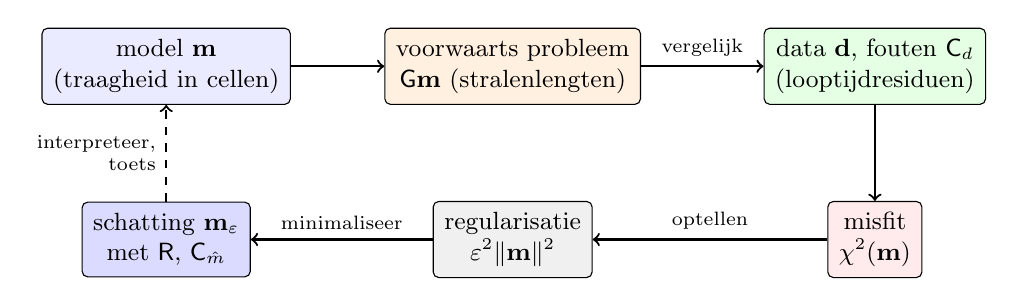
\begin{tikzpicture}[font=\small, node distance=0.5cm,
  box/.style={draw, rounded corners=2pt, fill=#1, minimum height=0.9cm, align=center, inner sep=4pt},
  box/.default=gray!8]
\node[box=blue!8] (m) at (0,0) {model $\mathbf m$\\(traagheid in cellen)};
\node[box=orange!12] (g) at (4.4,0) {voorwaarts probleem\\$\mathsf G\mathbf m$ (stralenlengten)};
\node[box=green!10] (d) at (9.0,0) {data $\mathbf d$, fouten $\mathsf C_d$\\(looptijdresiduen)};
\node[box=red!8] (mis) at (9.0,-2.2) {misfit\\$\chi^2(\mathbf m)$};
\node[box=gray!12] (reg) at (4.4,-2.2) {regularisatie\\$\varepsilon^2\|\mathbf m\|^2$};
\node[box=blue!14] (est) at (0,-2.2) {schatting $\mathbf m_\varepsilon$\\met $\mathsf R$, $\mathsf C_{\hat m}$};
\draw[->, thick] (m) -- (g);
\draw[->, thick] (g) -- node[above, font=\scriptsize] {vergelijk} (d);
\draw[->, thick] (d) -- (mis);
\draw[->, thick] (mis) -- node[above, font=\scriptsize] {optellen} (reg);
\draw[->, thick] (reg) -- node[above, font=\scriptsize] {minimaliseer} (est);
\draw[->, thick, dashed] (est) -- node[left, font=\scriptsize, align=right] {interpreteer,\\toets} (m);
\end{tikzpicture}

\par\smallskip{\small Het lineaire \omterm{def:b3:seismology-imaging:inverse}{invers probleem} als lus (schematisch). Het
\omterm{def:b3:seismology-imaging:inverse}{voorwaarts probleem} voorspelt data uit een model; de misfit, gewogen met de
datafouten, meet de afwijking; de regularisatieterm houdt het model
klein; het minimaliseren van hun som levert de schatting op, die alleen
interpreteerbaar is samen met haar resolutiematrix en covariantie.}
\label{fig:b3:seismology-imaging:inverse-loop}
\end{omfigure}

\section{Seismische tomografie}\label{sec:b3:seismology-imaging:tomography}

\begin{definition}[Seismische tomografie, looptijdresidu]\label{def:b3:seismology-imaging:tomography}
Het \emph{looptijdresidu}\index{looptijdresidu} van een aankomst is de
waargenomen looptijd min de looptijd die een referentiemodel voorspelt,
$\delta t = T_{\text{obs}} - T_{\text{ref}}$, na correctie voor de
bronlocatie en oorsprongstijd, de hoogte van het station en de
ellipticiteit van de Aarde. \emph{Seismische tomografie}\index{seismische tomografie} is de
schatting van de driedimensionale afwijkingen van de seismische snelheden ten
opzichte van een referentiemodel, $\delta v(\mathbf x)$, uit een grote verzameling residuen (of
van golfvormen), door een \omterm{def:b3:seismology-imaging:inverse}{invers probleem} op te lossen.
\end{definition}

Schrijf $s = 1/v$ voor de traagheid. De looptijd langs een straal $\Gamma$ is
$T = \int_\Gamma s\,\mathrm dl$; maar de straal zelf hangt af van de snelheden,
waardoor het probleem niet-lineair lijkt. Het antwoord in de eerste orde is dat het
er niet toe doet.

\begin{proposition}[Gelineariseerd looptijdresidu]\label{prop:b3:seismology-imaging:linear}
Als de traagheid van het referentiemodel $s_0$ wordt verstoord tot $s_0 + \delta s$,
verandert de looptijd tussen twee vaste punten, tot op de eerste orde in
$\delta s$, met
\[
  \delta t = \int_{\Gamma_0}\delta s\,\mathrm dl ,
\]
waarbij de integraal wordt genomen langs de straal $\Gamma_0$ van het referentiemodel; de
relatieve snelheidsafwijking is $\delta v/v_0 = -\delta s/s_0$ van dezelfde orde.
\end{proposition}

\begin{proof}
Volgens het principe van Fermat maakt de straal $\Gamma_0$ de looptijd
$\int s_0\,\mathrm dl$ stationair ten opzichte van naburige paden: het verplaatsen van het pad over een
kleine hoeveelheid $\epsilon$ verandert de tijd alleen met een term van orde $\epsilon^2$.
De nieuwe straal $\Gamma$ verschilt van $\Gamma_0$ met een grootte van orde $\delta s$;
dus $\int_\Gamma(s_0 + \delta s)\,\mathrm dl = \int_{\Gamma_0}s_0\,\mathrm dl +
O(\delta s^2) + \int_{\Gamma_0}\delta s\,\mathrm dl + O(\delta s^2)$. Tot slot
$\delta(1/s) = -\delta s/s_0^2$, dus $\delta v/v_0 = -\delta s/s_0$.
\end{proof}

Verdeel het gebied in $M$ cellen met uniforme verstoring van de traagheid $\delta s_j$.
Het residu van straal $i$ wordt $\delta t_i = \sum_j L_{ij}\,\delta s_j$, waarbij
$L_{ij}$ de lengte is van de referentiestraal $i$ in cel $j$: een lineair \omterm{def:b3:seismology-imaging:inverse}{invers
probleem} waarvan de kern de matrix van stralenlengtes is, waarvan bijna alle elementen
nul zijn. De residuen zijn klein: in een mantel waar de snelheid \qty{8}{km.s^{-1}} is,
verkort een gebied van \qty{200}{km} breed dat \qty{3}{\percent}
sneller is, de looptijd van een verticale straal met ongeveer \qty{0.7}{s} (oefening 9).

\begin{method}[Looptijdtomografie]\label{met:b3:seismology-imaging:tomo}
\begin{enumerate}
  \item Kies de aankomsttijden van één fase (bijvoorbeeld P) bij alle stations, voor
        aardbevingen waarvan de locatie goed bekend is; bereken de residuen
        ten opzichte van een \omterm{def:b3:seismology-imaging:tables}{looptijdtabel}, gecorrigeerd voor de afplatting en
        de hoogte van het station.
  \item Teken de referentiestralen en verdeel het gebied in cellen (of ontwikkel
        $\delta s$ naar gladde functies); vul de matrix van stralenlengtes in.
  \item Ken aan elk residu zijn fout toe, afgeleid uit de nauwkeurigheid van het aflezen, en los
        het probleem van \omterm{def:b3:seismology-imaging:damped}{gedempte kleinste kwadraten} op voor een reeks dempingswaarden; teken
        de \omterm{def:b3:seismology-imaging:damped}{afwegingskromme} en kies de demping nabij het knikpunt.
  \item Toets de resolutie: bereken de residuen die een bekend synthetisch
        model via dezelfde stralen zou geven, voeg ruis toe, inverteer ze met dezelfde
        demping en vergelijk.
  \item Interpreteer alleen de afwijkingen die de test laat zien dat de stralen
        kunnen reconstrueren, waarbij hun amplitudes worden opgevat als ondergrenzen.
\end{enumerate}
\end{method}

\begin{definition}[Schaakbordtest]\label{def:b3:seismology-imaging:checkerboard}
Een \emph{schaakbordtest}\index{schaakbordtest} is een resolutietest waarin
het synthetische model een regelmatig patroon is van afwisselend snelle en langzame
cellen: synthetische residuen, berekend via de werkelijke stralengeometrie, met ruis
van dezelfde grootte als de werkelijke fouten, worden geïnverteerd met dezelfde parametrisatie en
demping. Waar het patroon wordt teruggevonden, kunnen structuren van die grootte
opgelost worden; waar het patroon wordt uitgesmeerd of verloren gaat, kan dat niet.
\end{definition}

De figuren hieronder voeren de test uit op een modeldoorsnede van \qty{800}{km} breed en
\qty{400}{km} diep, verdeeld in 128 cellen van \qty{50}{km}. Twintig bronnen liggen
langs de onderkant en tweeëndertig stations langs de bovenkant, en alleen de stralen binnen
\ang{45} van de verticale worden gebruikt: 480 stralen die allemaal steil omhoog gaan,
de geometrie van stralen van verre aardbevingen die onder een netwerk omhoog komen. De
synthetische model bestaat uit blokken van $2\times2$ cellen, \qty{3}{\percent} snel of langzaam
rond \qty{8}{km.s^{-1}}; de residuen bevatten Gauss-ruis van
\qty{0.05}{s}.
% figdata: tomo_checkerboard.py (invented geometry; no real data)

\begin{omfigure}
\begin{tikzpicture}
\begin{groupplot}[group style={group size=2 by 2, horizontal sep=0.9cm, vertical sep=1.25cm},
  width=0.46\linewidth, height=0.3\linewidth, xmin=0, xmax=800, ymin=0, ymax=400,
  axis on top, enlargelimits=false, tick label style={font=\scriptsize},
  title style={font=\small, yshift=-1ex},
  colormap={tomo}{rgb255(0cm)=(178,24,43); rgb255(1cm)=(244,165,130); rgb255(2cm)=(247,247,247); rgb255(3cm)=(146,197,222); rgb255(4cm)=(33,102,172)},
  point meta min=-4, point meta max=4]
\nextgroupplot[title={(a) synthetisch model}, ylabel={\scriptsize hoogte (km)}]
\addplot[matrix plot*, mesh/cols=16, point meta=explicit] table[x=x, y=y, meta=dv] {figdata/out/bachelor-3-tomo_checkerboard-true.dat};
\nextgroupplot[title={(b) een selectie van de 480 stralen}, colormap/blackwhite]
\addplot[gray!70!black, thin, unbounded coords=jump] table[x=x, y=y] {figdata/out/bachelor-3-tomo_checkerboard-rays.dat};
\addplot[only marks, mark=triangle*, mark size=1.6pt, black, clip=false] table[x=x, y=y] {figdata/out/bachelor-3-tomo_checkerboard-receivers.dat};
\addplot[only marks, mark=star, mark size=1.8pt, red!70!black, clip=false] table[x=x, y=y] {figdata/out/bachelor-3-tomo_checkerboard-sources.dat};
\nextgroupplot[title={(c) hersteld, $\varepsilon = \qty{3}{km}$}, ylabel={\scriptsize hoogte (km)}, xlabel={\scriptsize afstand (km)}]
\addplot[matrix plot*, mesh/cols=16, point meta=explicit] table[x=x, y=y, meta=dv] {figdata/out/bachelor-3-tomo_checkerboard-rec-low.dat};
\nextgroupplot[title={(d) hersteld, $\varepsilon = \qty{60}{km}$}, xlabel={\scriptsize afstand (km)},
  colorbar right, colorbar style={width=0.2cm, ytick={-4,-2,0,2,4}, ylabel={\scriptsize $\delta v/v$ (\%)}, tick label style={font=\scriptsize}}]
\addplot[matrix plot*, mesh/cols=16, point meta=explicit] table[x=x, y=y, meta=dv] {figdata/out/bachelor-3-tomo_checkerboard-rec-high.dat};
\end{groupplot}
\end{tikzpicture}

\par\smallskip{\small Een \omterm{def:b3:seismology-imaging:checkerboard}{schaakbordtest} (verzonnen geometrie). (a) Het
synthetische model: blokken van \qty{100}{km} breed, \qty{3}{\percent} snel (blauw) of
langzaam (rood). (b) De 20 bronnen (sterren), de 32
stations (driehoeken) en enkele van de stralen, alle binnen \ang{45} van de verticale. (c) Met
lichte demping worden de blokken gevonden, maar ruisachtig, met afwijkingen tot ongeveer
\qty{8}{\percent} waar weinig stralen kruisen (kleuren verzadigen bij
\qty{4}{\percent}). (d) Met zware demping is het patroon zuiver, maar de
amplitude is verminderd, vooral langs de zijranden, waar weinig stralen kruisen
en allemaal onder vergelijkbare hoeken.}
\label{fig:b3:seismology-imaging:checkerboard}
\end{omfigure}

\begin{omfigure}
\begin{tikzpicture}
\begin{axis}[omrecord, width=0.62\linewidth, height=0.42\linewidth,
  xlabel={modelnorm $\|\delta v/v\|$ (\unit{\percent})},
  ylabel={misfit $\|\mathsf G\mathbf m - \mathbf d\|$ (\unit{s})}, xmin=0, xmax=42, ymin=0, ymax=12]
\addplot[blue!70!black, thick] table[x=norm, y=misfit] {figdata/out/bachelor-3-tomo_checkerboard-tradeoff.dat};
\addplot[only marks, mark=*, mark size=1.8pt, red!70!black] coordinates {(38.84,0.862) (29.42,1.159)};
\node[font=\scriptsize, anchor=south, red!70!black] at (axis cs:38.84,1.3) {$\varepsilon = 3$};
\node[font=\scriptsize, anchor=east, red!70!black] at (axis cs:28.6,0.55) {$\varepsilon = 60$};
\draw[gray, dashed] (axis cs:0,1.095) -- (axis cs:42,1.095);
\node[font=\scriptsize, anchor=south west] at (axis cs:1,1.15) {verwacht door de ruis};
\draw[green!45!black, densely dotted] (axis cs:33.94,0) -- (axis cs:33.94,12);
\node[font=\scriptsize, anchor=north west, green!45!black] at (axis cs:34.2,11.8) {werkelijk model};
\node[font=\scriptsize, anchor=west] at (axis cs:14,10.5) {zware demping};
\node[font=\scriptsize, anchor=east] at (axis cs:41,3.2) {lichte demping};
\end{axis}
\end{tikzpicture}

\par\smallskip{\small De \omterm{def:b3:seismology-imaging:damped}{afwegingskromme} van de \omterm{def:b3:seismology-imaging:checkerboard}{schaakbordtest}, voor dempingswaarden
$\varepsilon$ van 0.1 tot \qty{1000}{km} (de kern is uitgedrukt in kilometers,
met gelijke fouten). Langs het vlakke deel kost meer demping vrijwel geen passing: het
model krimpt doordat het ruis kwijtraakt. De knik ligt waar de misfit stijgt door het
niveau dat de ruis alleen al verwacht, $\sigma\sqrt{480} = \qty{1.095}{s}$; de
twee gedempte modellen van de vorige figuur liggen aan weerszijden ervan, en de
norm van het werkelijke schaakbord, \qty{33.9}{\percent}, ligt daartussen. Voorbij de
knik verwijdert de demping structuur die de gegevens nodig hebben.}
\label{fig:b3:seismology-imaging:tradeoff}
\end{omfigure}

De test illustreert de drie beperkingen van elk tomografisch beeld. De resolutie
wordt bepaald door de stralen: waar alle stralen evenwijdig lopen, wordt een anomalie langs hen uitgesmeerd,
en een cel die door weinig stralen wordt gekruist, is nauwelijks beperkt. Demping verlaagt de
amplitudes: de teruggevonden anomalieën zijn ondergrenzen.
En het beeld hangt af van het referentiemodel en de parametrisatie: alleen de
afwijkingen ten opzichte van de referentie worden in kaart gebracht, en niets kleiner dan een cel.
Met deze voorbehouden tonen de globale P- en S-golfbeelden de slabs van het
Boek~3 (in het hoofdstuk over subductie) als plaatvormige snelle gebieden die vanaf de trogen
naar beneden lopen, sommige afplattend boven de 670-km-discontinuïteit, andere
de ondermantel indringend; en brede langzame gebieden onder de Stille Oceaan en
Afrika boven de kern, met smallere langzame kanalen onder sommige hotspots, de
kandidaten voor de mantelpluimen van hetzelfde boek.

\begin{inthefield}[Een breedbandstation en een plaatsing op de oceaanbodem]
\begin{minipage}[t]{0.55\linewidth}\vspace{0pt}
Een permanent breedbandstation is een rustige plek: de seismometer staat op een
betonnen pijler die vastgebout is aan vaste gesteente, in een ondergrondse kluis of een korte tunnel, onder een
thermisch schild, want een tochtvlaag of een verandering van enkele honderdsten van een graad
kantelt het instrument meer dan een verre aardbeving. De drie componenten,
verticaal, noord en oost, worden continu gedigitaliseerd en naar een datacentrum gestuurd
met een satelliettijdstempel. Om een gebied onder de oceaan in beeld te brengen, laat een meetteam
in plaats daarvan oceaanbodemseismometers vanaf een schip laten zakken: elk zinkt op een anker,
registreert een jaar lang op de zeebodem en komt naar het oppervlak terug wanneer het schip
terugkeert en een akoestisch signaal stuurt om het los te laten. De bemanning leest vervolgens de
klokdrift af, corrigeert de registraties en voegt duizenden aankomsten aan de
tomografie toe.
\end{minipage}\hfill
\begin{minipage}[t]{0.42\linewidth}\vspace{0pt}
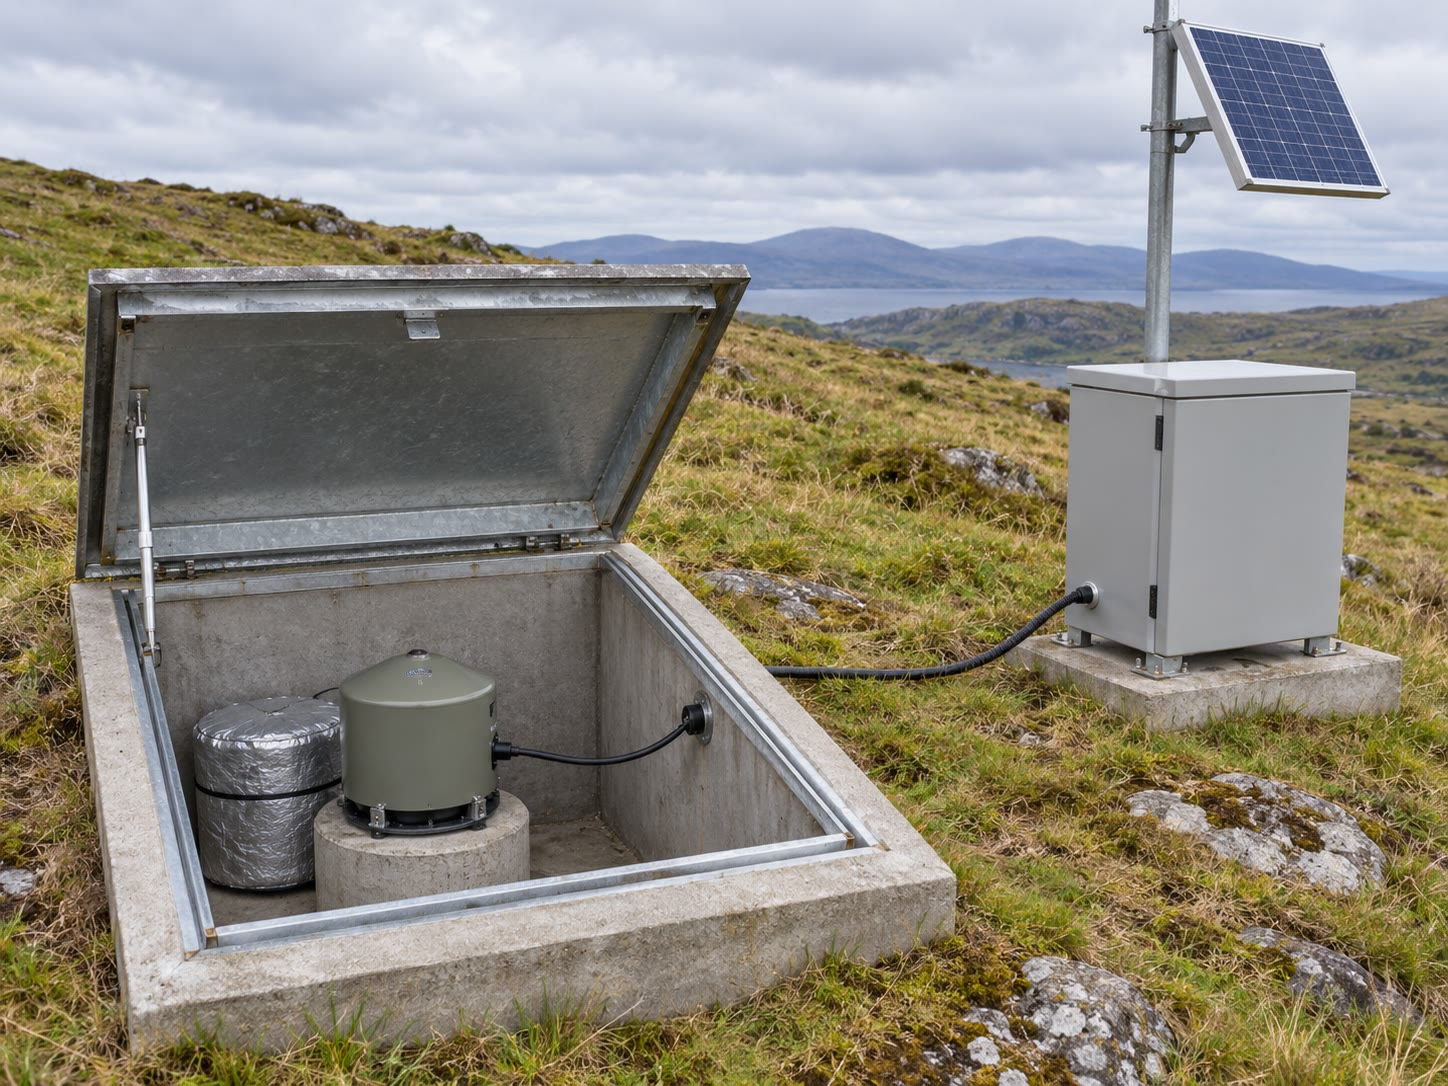
\includegraphics[width=\linewidth]{images/book5/ai/b3-seismic-vault.jpg}

{\scriptsize Een breedbandseismometer op zijn pijler in een stationskluis
(Door AI gegenereerde illustratie.)}
\end{minipage}
\end{inthefield}

\section{Oefeningen}

\begin{exercise}[$\star$]\label{exo:b3:seismology-imaging:1}
Een P-straal verlaat het oppervlak ($R = \qty{6371}{km}$, $v_0 = \qty{5.80}{km.s^{-1}}$)
met de \omterm{def:b3:seismology-imaging:ray-parameter}{straalparameter} $p = \qty{500}{s.rad^{-1}}$. (a) Bereken de
vertrekhoek. (b) PREM geeft P-snelheden van \qty{11.066}{km.s^{-1}} op \qty{771}{km} diepte
en \qty{11.245}{km.s^{-1}} op \qty{871}{km}. Bereken $r/v$ op beide dieptes en
bepaal de keerdiepte van de straal door lineaire interpolatie.
% ledger: ak135:crust, data:prem
\end{exercise}

\begin{exercise}[$\star$]\label{exo:b3:seismology-imaging:2}
De met PREM in dit hoofdstuk berekende P-looptijden bedragen \qty{369.6}{s} bij \ang{30}
en \qty{455.5}{s} bij \ang{40}. (a) Schat de helling van de looptijdkromme
ertussen, in \unit{s} per graad en in \unit{s.rad^{-1}}. (b) Leid hieruit
de schijnbare snelheid van het golffront langs het oppervlak af, in
\unit{km.s^{-1}}. (c) Wat is de P-snelheid op het keerpunt van de straal
die aankomt bij \ang{35}, als hij keert op de straal \qty{5450}{km}?
\end{exercise}

\begin{exercise}[$\star$]\label{exo:b3:seismology-imaging:3}
In het Lovegolfmodel van dit hoofdstuk heeft de laag $\beta_1 =
\qty{3.5}{km.s^{-1}}$, $\rho_1 = \qty{2700}{kg.m^{-3}}$ en de halfruimte
$\beta_2 = \qty{4.5}{km.s^{-1}}$, $\rho_2 = \qty{3300}{kg.m^{-3}}$.
(a) Bereken de twee afschuifmoduli. (b) Bij \qty{20}{s} is de fasesnelheid
\qty{3.79}{km.s^{-1}}: bereken de golflengte en vergelijk die met de laagdikte
\qty{35}{km}. (c) Met groepssnelheden van \qty{3.384}{km.s^{-1}} bij
\qty{20}{s} en \qty{4.333}{km.s^{-1}} bij \qty{100}{s}, hoeveel minuten komen de
golven van 20 s later aan dan die van 100 s bij een station op \qty{4000}{km} afstand?
\end{exercise}

\begin{exercise}[$\star$]\label{exo:b3:seismology-imaging:4}
De waargenomen perioden van ${}_0S_2$ en ${}_0T_2$ bedragen \qty{53.89}{min} en
\qty{44.01}{min}. (a) Bereken hun frequenties in \unit{mHz}. (b) Hoeveel
trillingen van elk maakt de Aarde in een dag? (c) Twee spectrale pieken
kunnen alleen worden gescheiden als de registratie minstens het omgekeerde van hun
frequentieverschil duurt. Hoe lang moet een registratie zijn om deze twee modi te scheiden?
% ledger: seis5:modes-S, seis5:modes-T
\end{exercise}

\begin{exercise}[$\star\star$]\label{exo:b3:seismology-imaging:5}
In een bol met straal $R$ en uniforme snelheid $v$ zijn de stralen rechte koorden.
(a) Toon aan dat de straal die $\Delta$ bereikt de looptijd
$T = 2R\sin(\Delta/2)/v$ heeft. (b) Met $R = \qty{6371}{km}$ en
$v = \qty{10.0}{km.s^{-1}}$, bereken $T$ bij \ang{30} en \ang{90}, en vergelijk
met de PREM-looptijden, \qty{369.6}{s} en \qty{779.7}{s}. (c) Verklaar waarom de
uniforme bol bij \ang{30} te snel en bij \ang{90} te langzaam is.
\end{exercise}

\begin{exercise}[$\star\star$]\label{exo:b3:seismology-imaging:6}
Op een Poissonvaste stof ($\lambda = \mu$, dus $\alpha^2 = 3\beta^2$) geldt voor de
snelheid $c$ van de \omterm{def:b3:seismology-imaging:surface-waves}{Rayleighgolf}, met $\xi = c^2/\beta^2$,
$(2 - \xi)^2 = 4\sqrt{1 - \xi/3}\,\sqrt{1 - \xi}$. (a) Kwadrateer dit en toon
aan dat de wortels voldoen aan $(\xi - 4)(3\xi^2 - 12\xi + 8) = 0$. (b) Toon aan dat de
enige wortel met $0 < \xi < 1$ gelijk is aan $\xi = 2 - 2/\sqrt3$, en bereken $c/\beta$.
(c) In de bovenste korst van ak135 is $\beta = \qty{3.46}{km.s^{-1}}$: bereken de
Rayleighsnelheid en de vertraging van de \omterm{def:b3:seismology-imaging:surface-waves}{Rayleighgolf} ten opzichte van de S-golf bij
\qty{1000}{km}.
% ledger: ak135:crust
\end{exercise}

\begin{exercise}[$\star\star$]\label{exo:b3:seismology-imaging:7}
Kopgolfaankomsten bij vier stations van een refractielijn, op 50, 100, 150 en
\qty{200}{km} van het schot, zijn 9.0, 15.3, 21.5 en \qty{27.9}{s}, met
fouten van 0.1, 0.1, 0.2 en \qty{0.2}{s}. Pas $T = a + bx$ aan met gewogen kleinste kwadraten:
schrijf $\mathsf G$ en $\mathsf C_d$ uit, stel de normaalvergelijkingen op, en
geef $a$, $b$, hun standaardfouten, de snelheid $1/b$ met zijn fout, en de
minimale $\chi^2$. Is de passing acceptabel?
\end{exercise}

\begin{exercise}[$\star\star$]\label{exo:b3:seismology-imaging:8}
Een straal kruist twee cellen, met lengtes \qty{30}{km} en \qty{40}{km}, en heeft
een residu van \qty{0.50}{s}. (a) Waarom is $\mathsf N = \mathsf G^{\mathsf T}
\mathsf G$ singulier? (b) Van de modellen die het residu exact passen, is het model
met de kleinste norm $\mathbf m = \mathsf G^{\mathsf T}(\mathsf G\mathsf
G^{\mathsf T})^{-1}\mathbf d$: bereken het. (c) Bereken de matrix
$\mathsf R = \mathsf G^{\mathsf T}(\mathsf G\mathsf G^{\mathsf T})^{-1}\mathsf G$
en haar spoor. (d) Als de werkelijke anomalie \qty{0.01}{s.km^{-1}} is in alleen
de eerste cel, wat wordt dan teruggevonden?
\end{exercise}

\begin{exercise}[$\star\star$]\label{exo:b3:seismology-imaging:9}
Een plakvormig gebied van de mantel is \qty{3}{\percent} sneller dan zijn omgeving,
waar $v = \qty{9.0}{km.s^{-1}}$. (a) Bereken het residu van een straal die
\qty{200}{km} ervan verticaal kruist, met \cref{prop:b3:seismology-imaging:linear},
en exact. (b) Idem voor een straal die een dikte van \qty{100}{km} ervan kruist
onder \ang{40} ten opzichte van de normaal op de plaat. (c) Hoe groot is de
relatieve fout van de linearisatie?
\end{exercise}

\begin{exercise}[$\star\star\star$]\label{exo:b3:seismology-imaging:10}
In \cref{thm:b3:seismology-imaging:love} bestaat een boventoon van orde $n$ alleen
bij perioden die kort genoeg zijn. (a) Toon aan dat bij zijn afsnijding de
fasesnelheid $\beta_2$ is en $kHq_1 = n\pi$. (b) Leid de afsnijhoekfrequentie
$\omega_n = n\pi\beta_1\beta_2/\bigl(H\sqrt{\beta_2^2 - \beta_1^2}\bigr)$ af.
(c) Bereken de afsnijperiode van de eerste boventoon voor het model van het
hoofdstuk ($H = \qty{35}{km}$, $\beta_1 = 3.5$, $\beta_2 = \qty{4.5}{km.s^{-1}}$).
(d) Toon aan dat de grondmodus geen afsnijding heeft en dat zijn fasesnelheid
naar $\beta_1$ gaat bij korte perioden.
\end{exercise}

\begin{exercise}[$\star\star\star$]\label{exo:b3:seismology-imaging:11}
Neem de straal van oefening 8, met eenheid datafout. (a) Toon aan dat, voor elke
$\varepsilon > 0$, $(\mathsf G^{\mathsf T}\mathsf G + \varepsilon^2\mathsf
I)^{-1}\mathsf G^{\mathsf T} = \mathsf G^{\mathsf T}(\mathsf G\mathsf
G^{\mathsf T} + \varepsilon^2\mathsf I)^{-1}$. (b) Leid de gedempte resolutiematrix
$\mathsf R_\varepsilon = \mathsf G^{\mathsf T}\mathsf G/(\|\mathbf g\|^2 +
\varepsilon^2)$ af, waarbij $\mathbf g = (30, 40)$, en haar spoor. (c) Bereken het
spoor en het dataresidu voor $\varepsilon^2 = 0$, 2500 en \num{10000}
(in \unit{km^2}). Beschrijf de afweging.
\end{exercise}

\begin{exercise}[$\star\star\star$]\label{exo:b3:seismology-imaging:12}
In de uniforme bol van oefening 5: (a) toon met
\cref{thm:b3:seismology-imaging:benndorf} aan dat $p(\Delta) = (R/v)\cos(\Delta/2)$,
en controleer dit tegen de definitie van $p$ (de vertrekhoek van een koorde).
(b) Toon aan dat de straal die $\Delta_1$ bereikt keert op $r_1 = R\cos(\Delta_1/2)$.
(c) Neem aan dat $\int_0^{\Delta_1}\operatorname{arccosh}\bigl(\cos(\Delta/2)
/\cos(\Delta_1/2)\bigr)\,\mathrm d\Delta = \pi\ln\bigl(1/\cos(\Delta_1/2)\bigr)$,
toon aan dat de formule van Herglotz--Wiechert $r_1$ en de snelheid $v$ teruggeeft.
\end{exercise}

\section{Probleem: De plaat onder station K}

\begin{problem}[{Weekendprobleem --- stralen, Lovegolven en een kleine tomografie
onder een verzonnen station}]
\label{pb:b3:seismology-imaging:1}
% values: calc/ch01.py (invented station and models; Love-wave model as in the chapter)
Station K staat op een continent boven een subductiezone. Dit probleem gebruikt
zijn registraties op drie manieren: stralen in zijn korst, de dispersie van
Lovegolven erdoorheen, en een kleine tomografie van de mantel eronder.

\medskip
\noindent\textbf{Deel I --- Stralen in een gradiënt.} Over afstanden die kort
genoeg zijn om de kromming van de Aarde te verwaarlozen, neemt de P-snelheid onder
K lineair toe met de diepte, $v(z) = v_0 + gz$, met $v_0 = \qty{5.0}{km.s^{-1}}$ en
$g = \qty{0.05}{s^{-1}}$ ($z$ in km).
\begin{enumerate}
  \item In vlakke lagen behoudt de wet van Snellius $p = \sin i/v$ constant. Een
        straal vertrekt uit K met $\sin i_0 = 0.8$: bereken $i_0$ en $p$.
  \item Op welke diepte keert hij, en wat is de snelheid daar?
  \item Toon aan dat $\mathrm di/\mathrm ds = pg$ langs de straal, zodat het een
        cirkelboog is; geef de straal ervan en de diepte van zijn middelpunt.
  \item Bereken de horizontale afstand $X$ waarop de straal terugkeert naar het
        oppervlak.
  \item Toon aan dat $\mathrm dT = \mathrm di/(g\sin i)$ en bereken de looptijd
        $T$ exact.
  \item Bereken $X$ en $T$ voor $p = \qty{0.15}{s.km^{-1}}$, en controleer dat
        $\Delta T/\Delta X$ tussen de twee stralen ligt tussen de twee waarden
        van $p$.
\end{enumerate}

\noindent\textbf{Deel II --- Lovegolven en de korst.} De korst onder K is een
laag met S-snelheid $\beta_1 = \qty{3.5}{km.s^{-1}}$ en dichtheid
$\rho_1 = \qty{2.7}{g.cm^{-3}}$ op een mantel met $\beta_2 =
\qty{4.5}{km.s^{-1}}$, $\rho_2 = \qty{3.3}{g.cm^{-3}}$; zijn dikte $H$ is
onbekend. Tussen K en een buurstation wordt de fasesnelheid van de \omterm{def:b3:seismology-imaging:surface-waves}{Lovegolf}
gemeten: \qty{3.99}{km.s^{-1}} bij \qty{25}{s} en \qty{4.25}{km.s^{-1}} bij
\qty{40}{s}.
\begin{enumerate}[resume]
  \item Bereken $\mu_1$ en $\mu_2$ in \unit{GPa}.
  \item Bereken bij \qty{25}{s} $k$, $q_1$ en $q_2$.
  \item Los de dispersievergelijking van de grondmodus op voor $H$.
  \item Doe hetzelfde bij \qty{40}{s}. Zijn de twee resultaten consistent?
  \item Schat de groepssnelheid tussen de twee perioden als
        $\Delta\omega/\Delta k$, en vergelijk die met de fasesnelheden.
  \item Bereken de golflengte bij elke periode, en verklaar waarom de twee
        perioden de korst en de bovenste mantel in verschillende verhoudingen
        voelen.
\end{enumerate}

\noindent\textbf{Deel III --- Een tomografie in vier cellen.} Onder K is een blok
mantel van \qty{200}{km} bij \qty{200}{km} in een verticale doorsnede in vier
vierkante cellen van \qty{100}{km} verdeeld: 1 (linksboven), 2 (rechtsboven), 3
(linksonder) en 4 (rechtsonder); de trog en de oceaan liggen links. De referentiesnelheid is $v_0 = \qty{8.0}{km.s^{-1}}$. In een
geïdealiseerd experiment kruisen zes rechte stralen het blok: A langs de bovenste
rij (cellen 1 en 2), B langs de onderste rij (3 en 4), C langs de linkerkolom (1 en
3), D langs de rechterkolom (2 en 4), E langs de diagonaal door 1 en 4, F langs de
diagonaal door 2 en 3. Hun residuen zijn:
\begin{center}
\small
\begin{tabular}{lcccccc}
\hline
straal & A & B & C & D & E & F \\
$\delta t$ (\unit{s}) & $0.16$ & $-0.48$ & $-0.36$ & $0.11$ & $-0.15$ & $-0.27$ \\
fout $\sigma$ (\unit{s}) & 0.05 & 0.05 & 0.05 & 0.05 & 0.10 & 0.10 \\
\hline
\end{tabular}
\end{center}
Neem het model $\mathbf m$ als de traagheidsafwijkingen van de cellen in
\unit{ms.km^{-1}} ($\qty{1}{ms.km^{-1}} = \qty{e-3}{s.km^{-1}}$), zodat de
elementen van $\mathsf G$ de stralenlengtes in \unit{km} gedeeld door 1000 zijn.
\begin{enumerate}[resume]
  \item Schrijf $\mathsf G$ uit, een $6\times4$-matrix.
  \item Toon aan dat $\mathsf N = \mathsf G^{\mathsf T}\mathsf C_d^{-1}\mathsf G$
        de rijen $(10, 4, 4, 2)$, $(4, 10, 2, 4)$, $(4, 2, 10, 4)$,
        $(2, 4, 4, 10)$ heeft.
  \item Bereken $\mathbf b = \mathsf G^{\mathsf T}\mathsf C_d^{-1}\mathbf d$.
  \item Controleer dat $(1,1,1,1)$, $(1,-1,-1,1)$, $(1,1,-1,-1)$ en $(1,-1,1,-1)$
        eigenvectoren van $\mathsf N$ zijn, met eigenwaarden 20, 4, 8 en 8, en
        leid af dat $\mathsf N^{-1}$ de rijen $(11, -4, -4, 1)/80$,
        $(-4, 11, 1, -4)/80$, $(-4, 1, 11, -4)/80$ en $(1, -4, -4, 11)/80$ heeft.
  \item Bereken de \omterm{thm:b3:seismology-imaging:wls}{gewogen kleinstekwadratenschatting} $\hat{\mathbf m}$.
  \item Zet die om in relatieve snelheidsafwijkingen $\delta v/v_0$ in procent.
  \item Geef de standaardfout van elke cel in \unit{ms.km^{-1}} en in procent,
        en de correlatie tussen cel 1 en 2, en tussen cel 1 en 4. Verklaar hun
        tekens.
  \item Bereken de residuen van de zes stralen na de fit en de minimale
        $\chi^2$. Is die consistent met de opgegeven fouten?
\end{enumerate}

\noindent\textbf{Deel IV --- Demping, resolutie en de plaat.}
\begin{enumerate}[resume]
  \item Geef voor $\varepsilon^2 = 4$ (in de eenheden van $\mathsf N$) de
        eigenwaarden van $\mathsf R = (\mathsf N + 4\mathsf I)^{-1}\mathsf N$ en
        toon aan dat $\mathsf R$ de diagonaal $2/3$ heeft, de elementen $1/12$
        tussen cellen die een rij- of kolomstraal delen, en $0$ tussen cel 1 en 4
        en tussen cel 2 en 3.
  \item Bereken de gedempte schatting van cel 3 en haar snelheidsafwijking. Waarom
        is die kleiner dan de ongedempte?
  \item Het gedempte model heeft $\chi^2 = 15.8$ en norm \qty{2.91}{ms.km^{-1}};
        het ongedempte $\chi^2 = 0.50$ en \qty{4.24}{ms.km^{-1}}. Welk zou je
        houden, en waarom heeft dit probleem geen demping nodig?
  \item Lees rij 3 van de gedempte $\mathsf R$: met welke cellen is de schatting
        van cel 3 uitgesmeerd?
  \item Welke cel is snel, en welke langzaam? Interpreteer de snelle cel, onder en
        aan de oceaankant van K, in termen van de subductiezone.
  \item Geef de P-snelheidsafwijking van de plaatcel in procent, met haar
        standaardfout.
\end{enumerate}
\end{problem}
